\documentclass[border=6pt]{standalone}
\usepackage{garamondx}
\usepackage{pgfplots}
\usepackage{tikz}
\usepgfplotslibrary{units}
\usepackage{xcolor}
\definecolor{redtea}{rgb}{0.6823529412,0.2792156863,0.2666666667}
\usepackage{siunitx}
\usepackage{changepage}
\usepackage{calc}
\pgfplotsset{samples}
\usepgfplotslibrary{fillbetween}
\usetikzlibrary{backgrounds}
\pgfdeclarelayer{bg}
\pgfdeclarelayer{fg}
\pgfsetlayers{bg,main,fg}
\usetikzlibrary{patterns}


\begin{document}
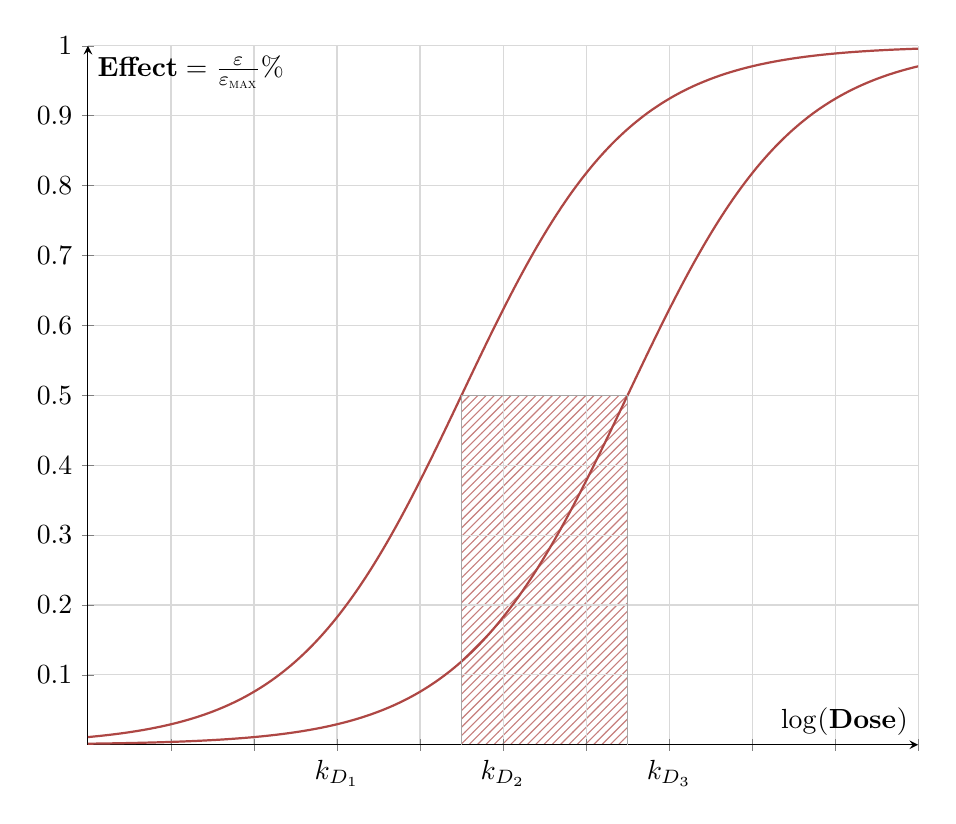
\begin{tikzpicture}
\begin{axis}[
width=\linewidth,
grid=major,
grid style={gray!30},
axis lines=middle,
xmax=10,
xmin=-0,
ymin=-0,
ymax=1,
xlabel={\scshape $\mathbf{\log}$(\textbf{Dose})},
ylabel={\scshape \textbf{Effect}$\;=\frac{\varepsilon}{\varepsilon_{\text{max}}}\%$},
xtick={1,2,3,4,5,6,7,8,9,10},
xticklabels={,,$k_{D_1}$,,$k_{D_2}$,,$k_{D_3}$,,,}
]
\addplot[redtea] [thick,smooth,domain=-0:30,samples=1000] {1/(1+exp(-1*(x-4.5)))};
\addplot[redtea] [thick,smooth,domain=-0:30,samples=1000] {1/(1+exp(-1*(x-6.5)))};
\end{axis}

\coordinate (a1) at (0,4.44);
\coordinate (a2) at (4.746,4.44);
\coordinate (a3) at (4.746,0);
\coordinate (a4) at (6.85,4.44);
\coordinate (a5) at (6.85,0);

%\draw[dashed,thick] (a1) to (a2);
\draw[gray!70] (a2) to (a3);
\draw[gray!70] (a2) to (a4);
\draw[gray!70] (a4) to (a5);

\begin{pgfonlayer}{bg}
\fill[pattern=north east lines, pattern color=redtea!70] (a2) -- (a4) -- (a5) -- (a3);
\end{pgfonlayer}


\end{tikzpicture}
\end{document}
